\chapter{Programación básica e intermedia}

\section{Número par / impar}

\enunciado{Desarrolle un programa que determine si un número es par o impar.}

\sol

Este ejercicio es uno de los más comunes en los cursos básicos de programación. 
Para resolverlo hay que tener en cuenta algunas nociones básicas de matemáticas: es 
sabido que cualquier número par es divisible por 2, lo cual nos lleva al supuesto de que 
si un número es par necesariamente el resto de la división entre 2 debe ser igual a cero. 
La función rem de MATLAB devuelve 0 si el residuo de la división entera es nulo, y devuelve 1 
si es una cantidad igual o mayor a la unidad. Basándonos en lo anterior podemos diseñar 
un programa que ejecuta la comprobación y que muestre en pantalla si el número es par o impar.

\begin{verbatim}
num=input('Numero: ');
if rem(num,2)==0
    disp('Numero par');
else
    disp('Numero impar');
end
\end{verbatim}

El programa anterior utiliza la sentencia compuesta if-else para llevar a cabo dicha tarea. 
Es posible también usar la sentencia switch tal como se muestra enseguida, los resultados, desde luego, son iguales.

\begin{verbatim}
num=input('Numero: ');
switch rem(num,2)
    case 0
        disp('Numero par');
    otherwise
        disp('Numero impar');
end
\end{verbatim}

% ------------------------------------------------------------------------------------------------

\section{Lista de números pares}

\enunciado{Desarrolle un programa que proporcione los primeros números pares que se indiquen:}

\sol

Para desarrollar la solución a este problema se hará uso del operador {\it dos puntos}, el cual 
permite crear una lista o vector de valores numéricos con un cierto patrón, con la sintaxis:

\begin{verbatim}
v=a:h:b;
\end{verbatim}

Donde a es el valor inicial, h el incremento y b el valor final. En este caso necesitamos una lista 
de valores que comienze con el primer número par (2), con incrementos de 2, y cuyo valor final dependa 
de la cantidad de número pares requeridos. Por ejemplo, si se requieren 3 números pares, se esperaría que 
el último valor sea 6, que es equivalente a tener 2x3, así, de forma generalizada, el valor final será 
2n, donde n es la cantidad de números pares.

\begin{verbatim}
n=input('¿Cuantos numeros pares necesita? ');
pares=2:2:2*n;
disp(pares);
\end{verbatim}

% ----------------------------------------------------------------------------------------------------------

\section{Números primos} 

\enunciado{Escriba una función que le permita determinar si un número entero pasado como argumento 
es primo, en caso de serlo devolverá un valor lógico {\tt true} y un valor {\tt false} en caso contrario. 
(La función {\tt isprime} de MATLAB realiza la misma operación).}

\sol

Primero, sin tantos formalismos, un número primo es aquel cuyos únicos divisores son el uno y él mismo. 
Así, un programa básico puede estructurarse haciendo la comprobación, uno a uno, si cada número en el intervalo 
$[1, n]$ es divisor del número en cuestión. Si la cantidad de divisores es mayor a 2, entonces el número 
no es primo. Véase el código siguiente propuesto como solución:

\begin{verbatim}
function r = esprimo(n)
L=1:n;
if nnz(rem(n,L)==0)==2
    r=true;
else
    r=false;
end
end
\end{verbatim}

En resúmen: sea define un vector $L$ de $n$ elementos que contiene todos los números en el intervalo $[1,n]$, 
enseguida se aplica la función {\tt rem} a todos los elementos del vector $L$ y a esto se aplica la condición 
de ser igual a cero, resultando un vector de tipo lógico, donde los unos corresponden a aquellos números donde 
el residuo de la división entera es cero y por tanto divisores de $n$; finalmente, mediante la función 
{\tt nnz} se {\it cuentan} los elementos que no son ceros, si estos son igual a dos, entonces se tiene un 
número primo.

% -------------------------------------------------------------------------------------------------------

\section{Área y perímetro de un círculo}

\enunciado{Escriba un programa cuya entrada sea el radio del círculo e imprima el valor del área y 
perímetro correspondiente.}

\sol

Para resolver este problema, lo primero es remitirnos a los cursos de geometría básica y recordar 
que el área y perímetro (circunferencia) de un círculo vienen dados por:

$$A=\pi r^2$$
$$P=2 \pi r$$

Con lo anterior se plantea una solución:

\begin{verbatim}
radio=input('Radio del círculo: ');
area=pi*radio^2;
perimetro=2*pi*radio;
fprintf('Área: %g \n',area);
fprintf('Perímetro: %g \n',perimetro);
\end{verbatim}

% ============================================================================================================

\section{Conversión grados – radianes}

\enunciado{Utilice cualquier sentencia de selección múltiple para desarrollar un programa que le permita hacer la conversión de grados sexagesimales a radianes y viceversa.}

\sol

Sea $\theta_r$ un ángulo dado en radianes y $\theta_g$ en grados sexagesimales, las {\it formulas} de 
conversión resultan en:

$$\theta_r = \theta_g \left(\frac{\pi}{180}\right)$$
$$\theta_g = \theta_r \left(\frac{180}{\pi}\right)$$

\begin{verbatim}
opcion=input(['Seleccione una opción: \n 1. Grados a radianes'...
'\n 2. Radianes a grados \n']);
theta=input('Inserte la magnitud del angulo: ');
switch opcion
    case 1
        thetaR=theta*pi/180;
        fprintf('%g ° = %g rad \n',theta,thetaR);
    case 2
        thetaG=theta*180/pi;
        fprintf('%g rad = %g ° \n',theta,thetaG);
    otherwise
        disp('Opcion incorrecta');
end
\end{verbatim}


% ============================================================================================================
\section{Promedio de una lista de valores}

\enunciado{Realice un programa que pida la cantidad de elementos o datos a introducir y que posteriormente sean ingresados manualmente, con los datos anteriores calcular el promedio de los mismos.}

\sol

\begin{verbatim}
n=input('Cantidad de datos a introducir: ');
for i=1:n
    D(i)=input(['Dato ',num2str(i),': ']);
end
fprintf('El promedio de los datos introducidos es %g\n',mean(D));
\end{verbatim}


% ============================================================================================================
\section{Sucesión de Fibonacci}

\enunciado{Escriba un programa que imprima en pantalla los primeros n términos de la sucesión de Fibonacci.}

\sol

La sucesión de Fibonacci es una sucesión infinita de números naturales, cuyos términos resultan de la 
suma de los dos términos anteriores. Los primeros dos términos son 1 y 1, y enseguida el resto siguen 
el patrón descrito con anterioridad, así, algunos de los primeros términos se muestran enseguida:

$$ 1,1,2,3,5,8,13,21,34,55,... $$

Luego, cada término de la sucesión se calcula bajo la siguiente especificación: $f_i=f_{i-1}+f_{i-2}$. 
La implementación en MATLAB resulta muy sencilla, se definen inicialmente los dos primeros términos y 
enseguida se concatenan los valores de la sucesión que siguen el patrón mencionado, mediante un bucle. 
Un código de ejemplo se muestra a continuación:

\begin{verbatim}
n=input('Numero de terminos a mostrar: ');
F=[1 1];
for i=3:n
    F(i)=F(i-1)+F(i-2);
end
disp(F);
\end{verbatim}


% ============================================================================================================
\section{Múltiplos de un número}

\enunciado{Desarrolle una función que devuelva los primeros k múltiplos de un determinado número.}

\sol

Un múltiplo de un número es aquel que lo contiene un número entero de veces. Luego, los primeros $k$ 
múltiplos de un número $N$ cualesquiera, vienen dado por $<1,2,...,k-1,k>*N$. La implementación 
en MATLAB es muy sencilla, utilizando la notación de dos puntos para crear un vector cuyos elementos 
sean los enteros desde 1 hasta $k$.

\begin{verbatim}
function x = multiplos(num,k)
% Devuelve los primeros k multiplos de num.
%
x=(1:k)*num;
end
\end{verbatim}


% ============================================================================================================
\section{Ecuación cuadrática}

\enunciado{Escriba una función que le permita resolver una ecuación de segundo grado de la forma 
$ax^2+bx+c=0$, siendo los coeficientes los argumentos de entrada y las raíces de la ecuación los valores de salida.}

\sol

La solución general de una ecuación de segundo grado de la forma $ax^2+bx+c=0$ viene dada por la tan conocida 
{\bf formula general}.

$$x_{1,2}=\frac{-b\pm\sqrt{b^2-4ac}}{2a}$$

\begin{verbatim}
function [x1,x2]=ecuadratica(a,b,c)
% Resuelve una ecuacion de segundo orden, siendo
% los argumentos de entrada los coeficientes de
% la misma.
x1=(-b+sqrt(b^2-4*a*c))/(2*a);
x2=(-b-sqrt(b^2-4*a*c))/(2*a);
end
\end{verbatim}


\section{Tiempo de vida}

\enunciado{Desarrolle un script que le permita calcular el número de años, meses, días y horas que ha vivido un individuo.}

\sol

\begin{verbatim}
D=input('Día de nacimiento: ');
M=input('Mes de nacimiento: ');
A=input('Anio de nacimiento: ');
actual=now;
nac=datenum(A,M,D);
fprintf('\n¿Cuanto has vivido?\n');
fprintf('Anios = %g \n',(actual-nac)/365);
fprintf('Meses = %g \n',(actual-nac)/30);
fprintf('Dias = %g \n',(actual-nac));
fprintf('Horas = %g \n',(actual-nac)*24);
\end{verbatim}


% =========================================================================================================
\section{Adivinar el número}

\enunciado{Escriba un programa que genere un número entero aleatorio entre 1 y 100, y posteriormente le pida al usuario tratar de adivinar el número en cuestión, para cada intento el programa debe mostrar si el número que se trata de adivinar es mayor o menor al propuesto por el jugador. El programa termina cuando el jugador adivina el número, imprimiéndose en pantalla la cantidad de intentos realizados.}

\sol

Para generar el número entero aleatorio en el rango $[1,100]$ se utilizará la función \texttt{randi}, que devuelve un 
entero aleatorio en el intervalo que se especifique. Dentro de un bucle while se hacen las comprobaciones de equivalencia 
del número aleatorio con el número propuesto por el jugador. Además se utiliza un contador que se incrementa en la unidad 
cada vez que se ejecuta un ciclo. El ciclo se \textit{rompe} cuando el jugador adivina el número mediante la 
instrucción \texttt{break}.

\begin{verbatim}
n=randi([1 100]);
k=0;
while 1
    np=input('¿Numero?: ');
    k=k+1;
    if n<np
        disp('Es menor');
    elseif n>np
        disp('Es mayor');
    else
        break;
    end
end
fprintf('Lo has conseguido en %g intentos \n',k);
\end{verbatim}

% =========================================================================================================
\section{Imprimir rombo} 

\enunciado{Desarrolle un programa que imprima un rombo de asteriscos en pantalla para un valor 
dado de n, donde n es el número de filas y/o columnas totales del rombo, debe notar que n será 
siempre un entero impar mayor o igual 3. Para una mejor comprensión se muestran a continuación 
los resultados para n=3 y n=7.}

\begin{center}
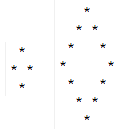
\includegraphics[scale=1]{src/rombo.png}
\end{center}

\sol

\begin{verbatim}
n=input('Numero de filas del rombo: ');
R='';
for i=1:n
    if i<=ceil(n/2)
        R(i,[ceil(n/2)+(1-i) ceil(n/2)+(i-1)])='*';
    else
        R(i,[ceil(n/2)-(n-i) ceil(n/2)+(n-i)])='*';
    end
end
disp(R);
\end{verbatim}

\section{Factorial de un número}

\enunciado{El factorial de un entero positivo n viene dado por $n!=(1)(2)...(n-1)(n)$, es decir, el producto 
de todos los enteros desde 1 hasta n. Realice un programa que devuelva el factorial de un número 
introducido (Recuerde que por definición el factorial de 0 es igual a la unidad).}

\sol

\begin{verbatim}
N=input('Introduzca un numero entero: ');
k=1;
fact=1;
while k<=N
    fact=k*fact;
    k=k+1;
end
fprintf('\n %d! = %d\n\n',N,fact);
\end{verbatim}


\section{Imprimir triángulo}

\enunciado{Realice un script que imprima en pantalla un triángulo de asteriscos, el programa debe tener como entrada el número de filas del triángulo.}

\sol

\begin{verbatim}
n=input('Numero de filas: ');
A='';
for i=1:n
    A(i,1:2:2*i)='*';
end
disp(A)
\end{verbatim}


\section{Sumatoria de n múltiplos de 5}

\enunciado{Escriba un programa que devuelva la suma de los primeros n múltiplos de 5, que además cumplan la condición de no ser múltiplos de 10.}

\begin{verbatim}
N=input('Multiplos a sumar: ');
suma=0;
mult=5;
k=0;
while k<N
    if rem(mult,10)
        suma=suma+mult;
        k=k+1;
    end
    mult=mult+5;
end
disp(suma);
\end{verbatim}

\section{Tabla de funciones trigonométricas}

\enunciado{Desarrolle un programa que imprima una tabla de valores para las funciones trigonométricas más comunes en el rango 0° a 45° (seno, coseno y tangente).}

\begin{verbatim}
fprintf('====================================\n');
fprintf('°    sin(x)      cos(x)      tan(x)\n');
fprintf('====================================\n');
for x=0:pi/180:pi/4
    fprintf('%0.0f \t %0.4f \t %0.4f \t %0.4f\n',...
        x*(180/pi),sin(x),cos(x),tan(x));
end
\end{verbatim}

\section{Tabla de multiplicar} 

\enunciado{Escriba un programa que pida al usuario un entero positivo del cual se desarrollará e imprimirá en pantalla su tabla de multiplicación del 1 al 10, por ejemplo:}

\begin{center}
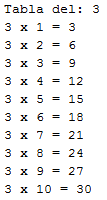
\includegraphics[scale=0.8]{src/tablamult.png}
\end{center}

\sol

\begin{verbatim}
N = input('Tabla del: ');
for k = 1:10
    fprintf('%g x %g = %g\n',N,k,N*k);
end
\end{verbatim}
